\sectionquestion{Neural Networks \& Backpropagation}

\begin{parts}


\part Consider the following dataset $\Dc_A = \{ (\xv^{(i)}, y^{(i)}) \}_{i=1}^4$:
\begin{center}
\begin{tabular}{|c|c|c|||c|}
\hline
$x_1^{(i)}$ & $x_2^{(i)}$ & $x_3^{(i)}$ & $y^{(i)}$ \\
\hline
0 & 0 & 1 & 0 \\
0 & 1 & 0 & 1 \\
1 & 0 & 0 & 1 \\
1 & 1 & 1 & 0 \\
\hline
\end{tabular}
\end{center}
Consider the following models:
\begin{itemize}
     %\item M1: feed polynomial functions of the raw features to a logistic regression model
     \item M1: feed linear combinations of the raw features to a logistic regression model
     %\item M3: use a 1-hidden-layer neural network with activation function $\sigma(a) = cos(a)$
     \item M2: use a 1-hidden-layer neural network with activation function $\sigma(a) = \frac{1}{1+exp(-a)}$
     \item M3: use a 1-hidden-layer neural network with activation function $\sigma(a) = w_1a + w_0$ where $w_i \in \Rb$
\end{itemize}
\begin{subparts}
\subpart[2] \textbf{Select all that apply:} Which of the following models has the potential to achieve zero training error on $\Dc_A$ without any additional feature engineering?

 {%
    \checkboxchar{$\Box$} \checkedchar{$\blacksquare$} % change checkbox style locally
    \begin{checkboxes}
     \choice M1
     \choice M2
     \choice M3
     \choice None of the above
    \end{checkboxes}
    }
    \begin{soln}
    all of the above, the dataset is linearly separable
    \end{soln}
    \begin{qauthor} Matt adapted from [insert name]'s question\end{qauthor}

\subpart[2] \textbf{Select all that apply:} Now suppose we remove the 3rd column from the dataset (i.e. feature $x_3^{(i)}$) to form $\Dc_B$. Which of the following models has the potential to achieve zero training error on $\Dc_B$ without any additional feature engineering?

 {%
    \checkboxchar{$\Box$} \checkedchar{$\blacksquare$} % change checkbox style locally
    \begin{checkboxes}
     \choice M1
     \choice M2
     \choice M3
     \choice None of the above
    \end{checkboxes}
    }
    \begin{soln}
    the dataset is not linearly separable; so only 
    (a) feed polynomial, (c) activation cosine, (d) activation sigmoid
    \end{soln}
    \begin{qauthor} Matt adapted from [insert name]'s question\end{qauthor}

% \subpart[2] What is a potential scenario in which this method will not result in separable data?
% \begin{soln}If we ever add different values of a new dimension to two points of the same value/label, then our data will never be linearly separable
% \end{soln}
\end{subparts}

\clearpage
\part Consider the following forward computation algorithm:
    \[
    \begin{aligned}
    & z = x \cdot y \\
    & a = z + y \\
    & b = z \cdot a \\
    & L = (b - t)^2
    \end{aligned}
    \]
where \( x, y \) are input nodes, \( z, a, b \)  are intermediate nodes, and \( L \) is the output node representing the loss and \( t \) is a target value. 
\begin{subparts}

\subpart[2] \textbf{Drawing:} Draw the corresponding \textbf{computation graph} diagram. For full credit, label each node with the corresponding variable and function.
\emph{Hint: recall that a computation graph diagram is not the same as a neural network diagram.}
        \begin{tcolorbox}[fit,height=5.5cm, width=15cm, blank, borderline={1pt}{-2pt}]
        %solution
        \end{tcolorbox} 
        \begin{soln}
            TODO
        \end{soln}

\subpart[4] \textbf{Fill in the blank:} Complete the psuedocode for the backpropagation algorithm below.
Your pseudocode should populate each variable $g_v$ with $\frac{\partial L}{\partial v}$, for all nodes $v$. You should reuse as much computation as possible. Your solution should \textbf{not} include any partial derivatives or partial derivative expressions. That is, your answer should be in terms of $x,y,z,a,b,t,L$ and $g_L, g_b, g_t, g_a, g_z, g_x, g_y$.

 \newcommand{\blankspace}{ \text{\underline{\phantom{$\frac{1}{2}$\hspace{18em}}}} }

\begin{align*}
            g_L &= \blankspace \\
            g_{b} &= \blankspace \\
            g_{t} &= \blankspace \\
            g_{a} &= \blankspace \\
            g_{z} &= \blankspace \\
            g_{x} &= \blankspace \\
            g_{y} &= \blankspace 
\end{align*}

% In the spirit of backpropagation, compute the following gradients only following through one step in the computation graph at a time i.e. you should express your answers only in a subset of variables specified and any constants you may need.
% \begin{itemize}
%         \item \( \frac{\partial L}{\partial b} = f(b, \hat{b}) = \rule{1cm}{0.15mm} \)
%         \item \( \frac{\partial L}{\partial a} = f(\frac{\partial L}{\partial b}, z) = \rule{1cm}{0.15mm} \)
%         \item \( \frac{\partial L}{\partial z} = f(\frac{\partial L}{\partial b}, \frac{\partial L}{\partial a}, z) = \rule{1cm}{0.15mm} \)
%         \item \( \frac{\partial L}{\partial x} = f(\frac{\partial L}{\partial z}, y) = \rule{1cm}{0.15mm} \)
%         \item \( \frac{\partial L}{\partial y} = f(\frac{\partial L}{\partial z}, \frac{\partial L}{\partial a}, x) = \rule{1cm}{0.15mm} \)
% \end{itemize}
    \begin{soln}

    \[
    g_L = 1
    \]
    \[
    g_b = g_L \cdot 2(b - t)
    \]
    \[
    g_t = g_L \cdot -2(b - t)
    \]
    \[
    g_a = g_b \cdot z
    \]
    \[
    g_z = g_b \cdot a + g_a
    \]
    \[
    g_x = g_z \cdot y
    \]
    \[
    g_y = g_z \cdot x + g_a
    \]
    \end{soln}
    \begin{qauthor}
    Yash, construct a computation graph for a function as specified by an algorithm, carry out the backpropagation on an arbitrary computation graph
    (adapted by Matt)
    \end{qauthor}

    
\end{subparts}

\newpage
\part[2] Suppose you are given the function $f(x) = 3x^2 + 2x + 5$ and you estimate it's derivative at $x = 2$ using the finite difference method with $\epsilon = 1$. 
Without referencing the exact value of the derivative at $x = 2$, do you think believe your estimate will be a good approximation of the true derivative? Briefly justify your answer in 1-2 concise sentences. 
\fillwithlines{6em}
\begin{soln}
    Probably not no, the value of $\epsilon$ used is very large relative to the function's scale. 
\end{soln}


\part 
Consider the following subpart of a neural network. The input $\xv$ is a vector of length 6 such that each element $x_i \in \{-1, 1\}$. 
%That is, $\xv \in \{1, -1\}^6$. 
The model weights are provided in the neural network diagram below. Assume the bias term is 0. 

\begin{minipage}{0.3\linewidth}
The activation function $\psi$ is given by:
\[
    \psi(a)= 
\begin{cases}
    1,& \text{if } a\geq 6\\
    0,              & \text{otherwise}
\end{cases}
\]
\end{minipage}
\begin{minipage}{0.7\linewidth}

\begin{center}
    \def\distH{2.1cm}
    \def\distHTwo{0.1cm}
    \def\distHThree{0.3cm}
    \def\distV{0.6cm}
    \def\distVTwo{0.3cm}
    \centering
    \begin{tikzpicture}[
        > = stealth, % arrow head style
        shorten > = 0pt, % don't touch arrow head to node
        auto,
        % node distance = 2.5cm, % distance between nodes
        thick % line style
    ]\footnotesize
    \tikzstyle{every state}=[
        draw = black,
        thick,
        fill = white,
        minimum size = 0.8cm,
    ]
    \node[state] (X1){$x_1$};
    \node[state] (X2) [right = \distV of X1] {$x_2$};
    \node[state] (X3) [right = \distV of X2] {$x_3$};
    \node[state] (X4) [right = \distV of X3] {$x_4$};
    \node[state] (X5) [right = \distV of X4] {$x_5$};
    \node[state] (X6) [right = \distV of X5] {$x_6$};
    \node[state] (Z1) [above left = \distH and \distVTwo of X4] {$z$};

    \path[->] (X1) edge node[pos=0.3, above, sloped] {$w_1 = 1$} (Z1);
    \path[->] (X2) edge node[pos=0.3, above, sloped] {$w_2 = 1$} (Z1);
    \path[->] (X3) edge node[pos=0.3, above, sloped] {$w_3 = 1$} (Z1);
    \path[->] (X4) edge node[pos=0.3, below, sloped] {$w_4 = -1$} (Z1);
    \path[->] (X5) edge node[pos=0.3, below, sloped] {$w_5 = -1$} (Z1);
    \path[->] (X6) edge node[pos=0.3, below, sloped] {$w_6 = -1$} (Z1);
    \end{tikzpicture}
    
\end{center}
\end{minipage}


\begin{subparts}
\subpart[2] \textbf{Numerical answer:} Write out an input $\xv$ such that the hidden unit is \emph{activated} (i.e., $z > 0$).

\begin{tcolorbox}[fit,height=1.5cm, width=15cm, blank, borderline={1pt}{-2pt}]
    %solution
\end{tcolorbox}
\begin{soln}
    only one possible answer: 
   $\xv = \begin{bmatrix}1 & 1 & 1 & -1 & -1 & -1\end{bmatrix}$ 
\end{soln} 

% REMOVED, non-essential
% \subpart[2] Although we can't compute the derivative of $\sigma(x)$ when $x = 6$, we can compute compute something else that is essential to training this model. What is its name?
%     \begin{tcolorbox}[fit,height=3cm, width=15cm, blank, borderline={1pt}{-2pt}]
%         %solution
%     \end{tcolorbox}
%     \begin{soln}
%         subderivative
%     \end{soln} 

\subpart[1] \textbf{Numerical answer:} Suppose all your data has the property that $x_1^{(i)} = x_4^{(i)}$, $x_2^{(i)} = x_5^{(i)}$, $x_3^{(i)} = x_6^{(i)}$, for all training examples $i$. With the weights initialized as shown above, what is $\psi(\wv^T \xv^{(i)})$ for an arbitrary $i$?
\begin{tcolorbox}[fit,height=1.5cm, width=4cm, blank, borderline={1pt}{-2pt}]
    %solution
\end{tcolorbox}
    \begin{soln}
    0
    \end{soln} 

\subpart[2] \textbf{Short answer:} Suppose our data has the same property as in the previous question. But now we replace $\psi(a)$ with a differentiable sigmoid $\psi'(a) = \frac{1}{1 + \exp(-1000(x-6))}$ such that $\psi'(a) \approx 1$ if $a > 6$ and $\psi'(a) \approx 0$ if $a < 6$. 
%
With the weights initialized as shown above, will training cause the weights $\wv$ to change quickly or slowly? \textbf{Briefly justify your answer.}
\fillwithlines{6em}
    \begin{soln}
        The gradient of the parameters will always be zero.
    \end{soln} 

\end{subparts}
\begin{qauthor}
   abbey. learning objectives: forward propagation / understanding how back propagation is done (gradient descent)
   
   Brynn Comments: This question seems good to me. I like that you have to understand NN but there is not much reading and the graph is clear.
   
   Matt: added two new subparts
\end{qauthor}



\begin{comment}
\part Consider the following dataset consisting of 6 data points in 2D space:

    \begin{minipage}{0.5\linewidth}
        \begin{center}
        \begin{tabular}{cc}
        \toprule
        \textbf{data point} & \textbf{label} \\ 
        \midrule
        (-1,1) & $+$ \\ 
        (1,1) & $-$ \\ 
        (-1,-1) & $-$ \\ 
        (1,-1) & $+$ \\ 
        (0,0) & $-$ \\
        (0,-0.5) & $+$ \\
        \bottomrule
        \end{tabular} 
        \end{center}
    \end{minipage}
    %
    \begin{minipage}{0.5\linewidth}
    \begin{tikzpicture}
    \begin{axis}[
        scatter/classes={
        a={mark=+,draw=black},
        b={mark=-,draw=black}}]
    \addplot[scatter,only marks,
        scatter src=explicit symbolic]
    table[meta=label] {
    x y label
    -1 1  a \\ 
    1 1   b \\ 
    -1 -1  b \\ 
    1 -1  a \\ 
    0 0  b \\
    0 -0.5 a \\
        };
    \end{axis}
    \end{tikzpicture}
    \end{minipage}

    \begin{subparts}

    \subpart[1] \textbf{Select one:} Does there exist a linear decision boundary that correctly classifies this dataset?     
    \begin{checkboxes}
     \choice Yes 
     \choice No
    \end{checkboxes}
    \begin{soln}
        N
    \end{soln}   
    
    \uplevel{Now, suppose you have a small neural network with one hidden layer, and sigmoid activations for both the hidden and output units.}

    \subpart[1] \textbf{Select one:} Does there exist a neural network of this form with just \textbf{two} neurons in the hidden layer that  correctly classifies this dataset? 
    \begin{checkboxes}
     \choice Yes 
     \choice No
    \end{checkboxes}
    \begin{soln}
        Y
    \end{soln}   
    
    \subpart[1] \textbf{Select one:} Does there exist a neural network of this form with just \textbf{three} neurons in the hidden layer that  correctly classifies this dataset? 
    \begin{checkboxes}
     \choice Yes 
     \choice No
    \end{checkboxes}
    \begin{soln}
        Y
    \end{soln}   
    
    \end{subparts}
    \begin{qauthor}
        Yash, a neural network can model nonlinear decision boundaries for classification
    \end{qauthor}
    \begin{qtester}
        I would need to draw this to fully test this, but otherwise seems like a good quick question
    \end{qtester}

\clearpage

\part[2] \textbf{Short Answer:} Neural the Narwhal decides to train a neural network to predict if a narwhal exists in an image. However, instead of using gradient descent to minimize the binary cross entropy of the network, he decides to use gradient ascent to maximize the training accuracy, where training accuracy is one minus training error. Is this likely to perform as well as the original? \textbf{Briefly justify your answer.}
    \begin{checkboxes}
     \choice Yes 
     \choice No
    \end{checkboxes}
    \fillwithlines{6em}
    \begin{soln}
    No. The accuracy is calculated by thresholding the prediction and is hence not differentiable. As it is not differentiable, backpropagation cannot be applied.
    \end{soln}
    \begin{qauthor}
        Advaith,
        Learning Objective: Identify when the gradient of a function can be computed at all and when it can be computed efficiently
    \end{qauthor}
    \begin{qtester}
        Maybe describe what the accuracy is in this case ($\frac{\# of examples classified correctly}{\# of examples}$). I thought that the question was considering that the the negative loss is the accuracy, in which case the answer would be yes.
    \end{qtester}


\part Consider an $n \times n$ matrix $\Av$ and length $n$ vector $\xv$.

    \begin{subparts}
    \subpart[1] \textbf{Short answer:} What is the shape of the derivative $\frac{d \Av \xv}{d \xv}$?
    \begin{tcolorbox}[fit,height=1cm, width=3cm, blank, borderline={1pt}{-2pt}]
    %solution
    \end{tcolorbox}
    \begin{soln}
    $n \times n$
    \end{soln}

  \subpart[2] \textbf{Short answer:} Compute the derivative $\frac{d \Av \xv}{d \xv}$. Your final answer may use $\Av$ and $\xv$, but you may not index into either.
    \begin{tcolorbox}[fit,height=2cm, width=6cm, blank, borderline={1pt}{-2pt}]
    %solution
    \end{tcolorbox}
    \begin{soln}
    $\Av^\top$
    \end{soln}
    \end{subparts}
    \begin{qauthor}
    Abhi, matrix calculus derivation, from recitation 5
    \end{qauthor}
    \begin{qtester}
        Seem fine, it's just calculus, but I would be interested in seeing who gets b incorrect.
    \end{qtester}

\part[2] \textbf{Short answer:} Consider some function $f(x)$. We wish to approximate the gradient of $f(x)$ at a given value $x_0$ using the finite difference method. Write an expression for the approximation of $f'(x_0)$ using the finite difference method. You may use $\epsilon$ to denote a small positive number.
    \begin{tcolorbox}[fit,height=2cm, width=6cm, blank, borderline={1pt}{-2pt}]
    %solution
    \end{tcolorbox}
    \begin{soln}
    Many possible answers. Example, $\dfrac{f(x_0 + \epsilon) - f(x_0 - \epsilon)}{2 \epsilon}$. Accept centered and non-centered.
    \end{soln}

    \begin{qauthor}
        Abhi, Use the finite difference method to evaluate the gradient of a function
    \end{qauthor}

    \begin{qtester}
        good question
    \end{qtester}

\clearpage

\part Consider a neural network that takes an input $[x_1, x_2]^T$, and returns a prediction $\hat{y} \in [0,1]$. Given a training example, $([x_1, x_2]^T, y^*)$ with $y^* \in \{0,1\}$, and parameters $\alpha \in \Rb, \beta \in \Rb$ we compute the loss $J \in \Rb$ following the algorithm below.
    \begin{center}
    \textbf{Forward Computation:}
    \begin{align*}
        a &= \alpha x_1 \\
        b &= \beta x_2 \\
        c &= a^2 \\
        d &= b\sin(a) \\
        \hat{y} &= c/d \\
        J &= \ell(\hat{y}, y^*) = \frac{1}{2}(y^* - \hat{y})^2
    \end{align*}
    \end{center}

 \begin{subparts}
    \subpart[3] \textbf{Drawing:} Draw the corresponding \textbf{computation graph} diagram. For full credit, label each node with the corresponding variable and function, and include everything from the input $[x_1, x_2]^T$ to the loss $J$.
        \emph{Hint: recall that a computation graph diagram is not the same as a neural network diagram.}
        \begin{tcolorbox}[fit,height=8cm, width=15cm, blank, borderline={1pt}{-2pt}]
        %solution
        \end{tcolorbox}
        \begin{soln}
        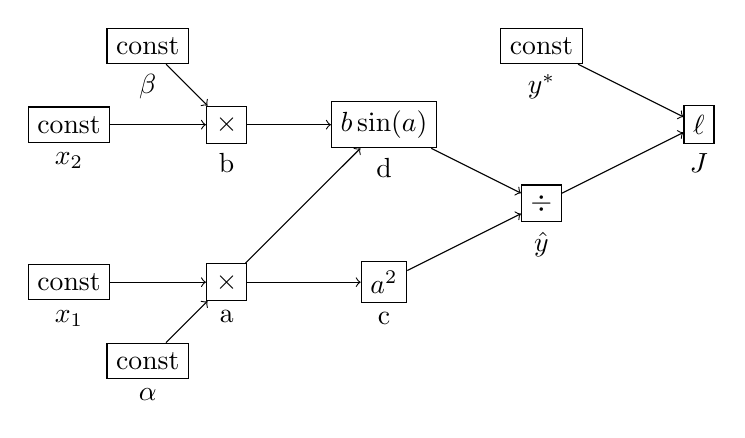
\begin{tikzpicture}
        
            \node[shape=rectangle,draw=black,label=below:$x_1$] (x1) at (0,0) {const};
            \node[shape=rectangle,draw=black,label=below:$x_2$] (x2) at (0,2) {const};
            \node[shape=rectangle,draw=black,label=below:$\alpha$] (alpha) at (1,-1) {const};
            \node[shape=rectangle,draw=black,label=below:$\beta$] (beta) at (1,3) {const};
            \node[shape=rectangle,draw=black,label=below:a] (a) at (2,0) {$\times$};
            \node[shape=rectangle,draw=black,label=below:b] (b) at (2,2) {$\times$};
            \node[shape=rectangle,draw=black,label=below:c] (c) at (4,0) {$a^2$};
            \node[shape=rectangle,draw=black,label=below:d] (d) at (4,2) {$b \sin(a)$};
            \node[shape=rectangle,draw=black,label=below:$\hat{y}$] (yhat) at (6,1) {$\div$};
            \node[shape=rectangle,draw=black,label=below:$y^*$] (ystar) at (6,3) {const};
            \node[shape=rectangle,draw=black,label=below:$J$] (J) at (8,2) {$\ell$};
    
            \path [->] (x1) edge (a);
            \path [->] (alpha) edge (a);
            \path [->] (x2) edge (b);
            \path [->] (beta) edge (b);
            \path [->] (a) edge (c);
            \path [->] (a) edge (d);
            \path [->] (b) edge (d);
            \path [->] (c) edge (yhat);
            \path [->] (d) edge (yhat);
            \path [->] (yhat) edge (J);
            \path [->] (ystar) edge (J);
        \end{tikzpicture}
        \end{soln}
        \begin{qauthor}
        Matt
        \end{qauthor}

\clearpage

    \subpart[4] \textbf{Fill in the blanks:} Complete the pseudocode for the backpropagation algorithm below. Your pseudocode should populate each variable $g_v$ with $\frac{\partial J}{\partial v}$, for all $v$. You should reuse as much computation as possible. Your solution should \textbf{not} include any partial derivatives or partial derivative expressions. That is, your answer should be in terms of $x_1, x_2, y^*, \alpha, \beta, a, b, c, d, \hat{y}, J$ and $g_{x_1}, g_{x_2}, g_{y^*}, g_{\alpha}, g_{\beta}, g_a, g_b, g_c, g_d, g_{\hat{y}}, g_J$ and any other numbers you may need.
    \newcommand{\blankspace}{ \text{\underline{\phantom{$\frac{1}{2}$\hspace{18em}}}} }

        \begin{center}
        \textbf{Backpropagation:}
        \begin{align*}
            g_J &= 1 \\
            g_{\hat{y}} &= \blankspace \\
            g_d &= \blankspace \\
            g_c &= \blankspace \\
            g_b &= \blankspace \\
            g_a &= \blankspace \\
            g_{\beta} &= \blankspace \\
            g_{\alpha} &= \blankspace 
        \end{align*}
        \end{center}
        
        \begin{soln}
        \textbf{Backpropagation:}
        \begin{align*}
            g_J &= 1 \\
            g_{\hat{y}} &= -g_J (y^* - \hat{y}) \\
            g_d &= g_{\hat{y}} (-\frac{c}{d^2}) \\
            g_c &= g_{\hat{y}} (\frac{1}{d}) \\
            g_b &= g_d (\sin(a)) \\
            g_a &= g_d (b \cos(a)) + g_c (2a) \\
            g_{\beta} &= g_b (x_2) \\
            g_{\alpha} &= g_a (x_1)
        \end{align*}
        \end{soln}
        \begin{qauthor}
        Matt
        \end{qauthor}
     
\end{subparts}    
\end{comment}

\end{parts}